\documentclass{article}
\usepackage{graphicx}
\usepackage{amsmath, amsfonts, amssymb}
\usepackage{enumitem}
\usepackage{wrapfig}
\usepackage{xcolor}
\usepackage{listings}
\usepackage{algorithm}
\usepackage{algpseudocode}
\usepackage{comment}
\usepackage[numbers]{natbib}
\usepackage{hyperref}
% minted needs pdflatex/latexmk run with -shell-escape (and pygments installed)
\usepackage{minted}
\usepackage{multirow}
\hypersetup{colorlinks=true, urlcolor=blue, citecolor=black, linkcolor=black}
\definecolor{LightGray}{gray}{0.9}
% global minted style applied to every \begin{minted} block below
\setminted{
    linenos,
    breaklines,
    frame=single,
    framesep=2mm,
    fontsize=\small,
    bgcolor=gray!1,
    tabsize=4
}
\title{Laplace Analysis and Applications}
% multi-author block: superscript numbers + a footnote-style affiliation list, no authblk needed
\author{
Pierre-Simon Laplace$^{1}$, Oliver Heaviside$^{2}$, and Gustav Robert Kirchhoff$^{3}$\\[6pt]
\small $^{1}$Acad\'emie des Sciences, Paris, France\\
\small $^{2}$Royal Society, London, United Kingdom\\
\small $^{3}$University of Heidelberg, Heidelberg, Germany
}
\date{}
\begin{document}
\maketitle
\section{From Functions to Transforms}
\subsection{The Laplace Transform}
Let $f(t)$ be a function defined for $t \geq 0$. Its Laplace transform is defined by
\begin{equation}
\mathcal{L}\{f(t)\} = F(s) = \int_{0}^{\infty} e^{-st} f(t)\,dt, \hspace{40px} s > 0.
\end{equation}
% \footnote attaches to the preceding word, numbered automatically
The transform changes a function of time into a function of the new variable s.\footnote{The variable s is commonly interpreted as a complex-frequency variable.} Symbolically,
$$ f(t) \xrightarrow{\mathcal{L}} F(s). $$
The Inverse Laplace transform reverses this process:
\begin{equation}
f(t) = \mathcal{L}^{-1} \{F(s)\}.
\end{equation}
The main purpose of the method is to replace differentiation and integration in the time domain
by simpler algebraic operations in the transform domain \cite{kreyszig2011}. A concise overview is available from
the \href{https://mathworld.wolfram.com/LaplaceTransform.html}{Laplace Transform entry on MathWorld}.
% \href{url}{display text} for a labeled hyperlink (vs. \url{...} for a raw one)
\subsection{A Simple Example}
For the constant function $f(t) = 1$,
% aligned (inside equation) lines up steps on & without a separate equation number per line
\begin{equation}
\begin{aligned}
\mathcal{L}\{1\}
&= \int_{0}^{\infty} e^{-st}\,dt \\
&= \left[-\frac{1}{s}e^{-st}\right]_{0}^{\infty} \\
&= \frac{1}{s}.
\end{aligned}
\end{equation}
Similarly,
\begin{equation}
\begin{aligned}
\mathcal{L}\{t\} = \frac{1}{s^2}, \hspace{20px} \mathcal{L}\{t^2\} = \frac{2}{s^3}.
\end{aligned}
\end{equation}
\section{Common Transform Equations}
% renewcommand{\arraystretch} below only affects this table's row height
Table~\ref{tab:laplace_transforms} lists several frequently used Laplace-transform equations.
\begin{table}[h]
\centering
\caption{Selected Laplace-transform equations.}
\label{tab:laplace_transforms}
\renewcommand{\arraystretch}{1.8} % Increases row height for fractions
% multirow for Family/Condition (spans the whole group), multicolumn + cline for the Transform Equation sub-header
\begin{tabular}{|c|c|c|c|}
\hline
\multirow{2}{*}{\textbf{Family}} & \multicolumn{2}{c|}{\textbf{Transform Equation}} & \multirow{2}{*}{\textbf{Condition}} \\
\cline{2-3}
& \textbf{Time function} & \textbf{Laplace transform} & \\
\hline
\multirow{3}{*}{Algebraic} & $1$ & $\dfrac{1}{s}$ & $s > 0$ \\
\cline{2-4}
& $t$ & $\dfrac{1}{s^2}$ & $s > 0$ \\
\cline{2-4}
& $t^n$ & $\dfrac{n!}{s^{n+1}}$ & $n = 0, 1, 2, \dots$ \\
\hline
\multirow{2}{*}{Exponential} & $e^{at}$ & $\dfrac{1}{s - a}$ & $s > a$ \\
\cline{2-4}
& $e^{-at}$ & $\dfrac{1}{s + a}$ & $s > -a$ \\
\hline
\multirow{2}{*}{Oscillatory} & $\sin(\omega t)$ & $\dfrac{\omega}{s^2 + \omega^2}$ & $\omega > 0$ \\
\cline{2-4}
& $\cos(\omega t)$ & $\dfrac{s}{s^2 + \omega^2}$ & $\omega > 0$ \\
\hline
\multicolumn{2}{|c|}{\textbf{Unit-step function } $u(t - a)$} & $\dfrac{e^{-as}}{s}$ & $a > 0$ \\
\hline
\end{tabular}
\end{table}
The formulas in Table~\ref{tab:laplace_transforms} allow many functions to be transformed without repeatedly evaluating
improper integrals.
\section{Application to an RC Circuit}
\subsection*{Circuit Model}
% wrapfigure{r}{width}: image pinned to the right, body text wraps around it
\begin{wrapfigure}{r}{0.5\textwidth}
    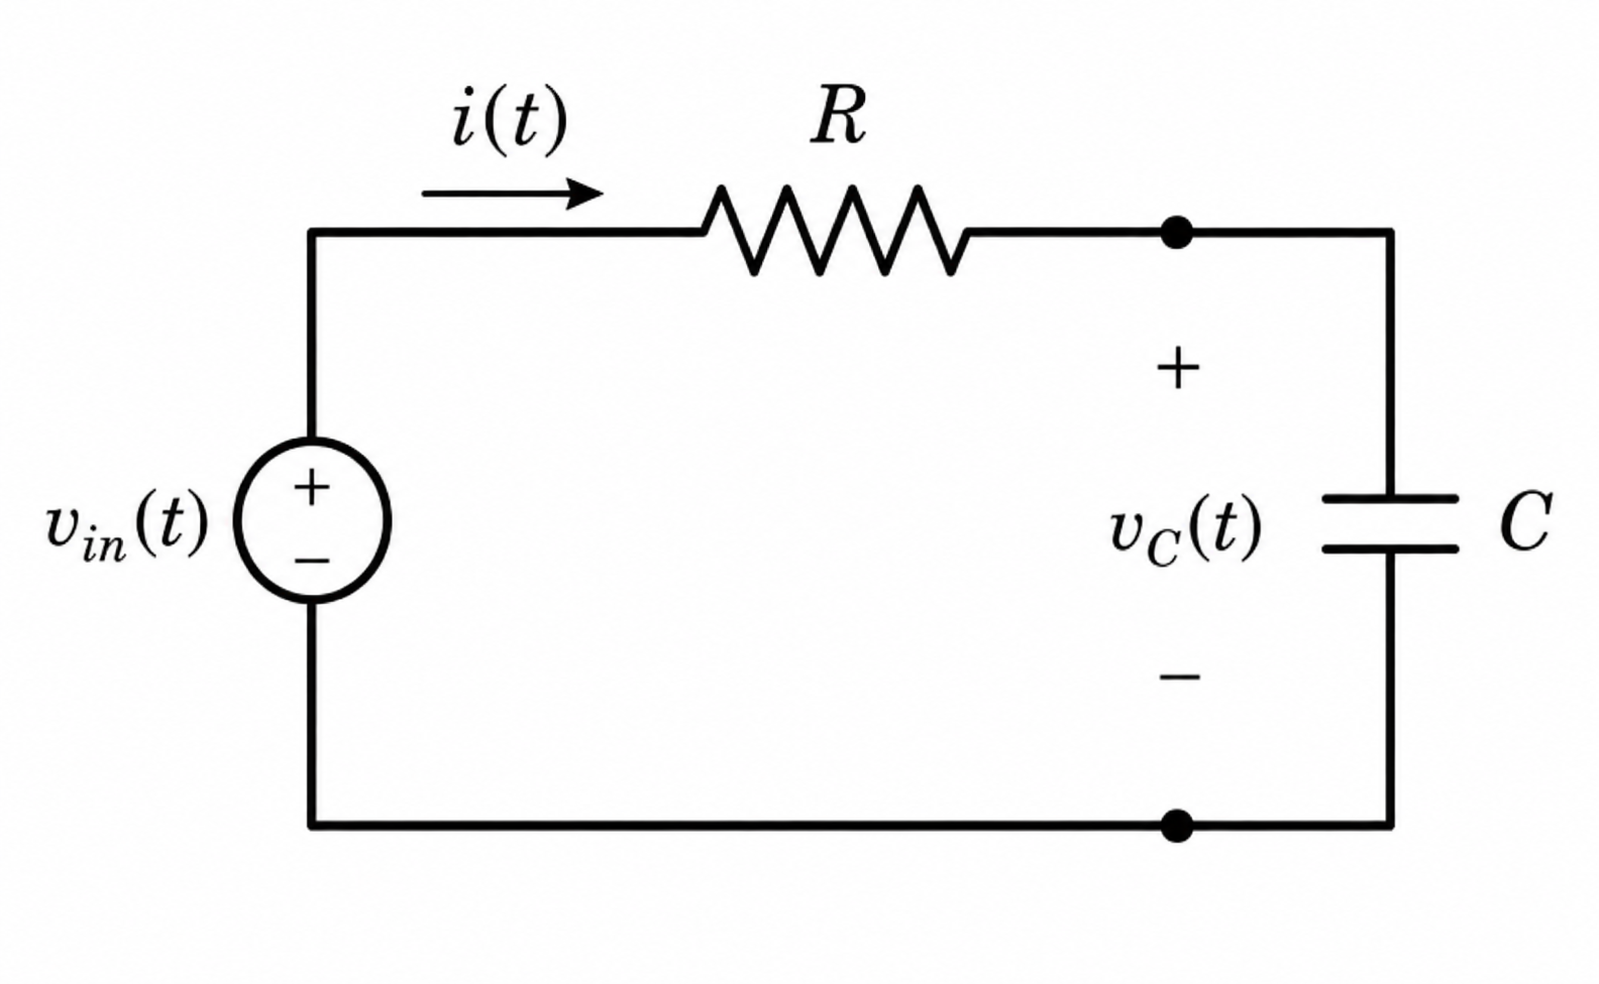
\includegraphics[width=0.5\textwidth]{rc_circuit.png}
    \caption{A simple series RC circuit.}
    \label{fig:rc_circuit}
\end{wrapfigure}
Figure~\ref{fig:rc_circuit} shows a \texttt{simple resistor--capacitor circuit} connected to an input voltage source.
The resistor limits the current, while the capacitor stores electrical energy.
For a resistor R and capacitor C, Kirchhoff's voltage law gives
\begin{equation}
    RC\dfrac{dv_{C}(t)}{dt} + v_{C}(t) = v_{in}(t), \label{eq:rc_ode}
\end{equation}
where $v_{C}(t)$ is the voltage across the capacitor.
Assuming $v_{C}(0) = 0$, taking the Laplace transform of Equation~\eqref{eq:rc_ode} gives
% align + nested split: one shared equation number for the whole derivation block
\begin{align}
    \begin{split}
    RC \left[ sV_{C}(s) - v_{C}(0) \right] + V_{C}(s) &= V_{in}(s),  \\
    \implies RCsV_{C}(s) + V_{C}(s) &= V_{in}(s), \\
    \implies V_{C}(s)(RCs + 1) &= V_{in}(s).
    \end{split}
    \label{eq:laplace_process}
\end{align}
The transfer function is therefore
\begin{equation}
    H(s) = \frac{V_{C}(s)}{V_{in}(s)} = \frac{1}{RCs+ 1}.
    \label{eq:transfer_function}
\end{equation}
For a constant input $V_0$,
\[
    V_{\mathrm{in}}(s) = \frac{V_0}{s}.
\]
Thus,
\begin{equation}
    V_C(s) = \frac{V_0}{s(RCs + 1)}.
    \label{eq:vc_step}
\end{equation}
Taking the inverse transform gives
\begin{equation}
    v_{C}(t) = V_{0} \left( 1 - e^{-t/(RC)} \right).
    \label{eq:vc_time}
\end{equation}
The quantity $\tau = RC$ is called the time constant of the circuit. A larger value of $\tau$ causes the capacitor to charge more slowly\cite{ogata2010}.
\section{How Laplace Analysis Is Used}
The Laplace transform is useful in many areas:
% label= removes the bullet so \textbf{...} below acts as a run-in heading; $\oplus$/$\rhd$ are symbol sub-labels
\begin{itemize}[leftmargin=*,label=]
    \item \textbf{Differential equations} $\oplus$ initial conditions are included automatically; \\
$\oplus$ derivatives become algebraic expressions.
    \item \textbf{Electrical circuits} $\oplus$ voltages and currents are studied in the s-domain; \\
$\oplus$ components lead to transfer functions.
    \item \textbf{Control and signal systems} $\oplus$ stability can be studied through poles; \\
$\oplus$ common test inputs include:
        \begin{itemize}
            \item[$\rhd$]  the unit-step input;
            \item[$\rhd$]  the impulse input;
            \item[$\rhd$]  sinusoidal inputs.
        \end{itemize}
\end{itemize}
% textcolor wraps a run of text, unlike \color which switches color until the next group ends
\textcolor{blue}{In the time domain, a system may be described by a differential equation}, whereas \textcolor{red}{in the Laplace
domain, the same system is often described by a rational algebraic expression.}
\section{A Short Python Implementation}
Listing~\ref{lst:rc_response} evaluates the capacitor voltage at a finite set of time instants using an external Python
file.
\begin{listing}[ht]
% minted{python} gives syntax-highlighted, line-numbered code per the \setminted options above
\begin{minted}{python}
from math import exp
def rc_response(resistance, capacitance, input_voltage, times):
    """Return capacitor-voltage samples for an RC step input."""
    if resistance <= 0 or capacitance <= 0:
        raise ValueError("R and C must be positive")
    tau = resistance * capacitance
    values = []
    for time in times:
        voltage = input_voltage * (1 - exp(-time / tau))
        values.append(voltage)
    return values
times = [0.0, 0.5, 1.0, 2.0]
print(rc_response(2.0, 0.5, 5.0, times))
\end{minted}
\caption{Computing samples of the RC step response.}
\label{lst:rc_response}
\end{listing}
Equation~\eqref{eq:vc_time} and Listing~\ref{lst:rc_response} describe the same computation.

% bibliographystyle + bibliography{name} (no .bib extension) pulls entries cited via \cite{...} above
\bibliographystyle{ieeetr}
\bibliography{laplace}
\end{document}